\documentclass[a4paper,11pt]{book}
\usepackage{listings}
\usepackage{xspace}
\usepackage{url}
\usepackage[utf8]{inputenc}
\usepackage[spanish]{babel}
\usepackage{pdfpages}

\decimalpoint
\usepackage{dcolumn}
\newcolumntype{.}{D{.}{\esperiod}{-1}}
\makeatletter
\addto\shorthandsspanish{\let\esperiod\es@period@code}
\makeatother

\RequirePackage{verbatim}
\usepackage{fancyhdr}
\usepackage{graphics, graphicx, float}
\usepackage{afterpage}

\usepackage{longtable}

\usepackage[pdfborder={000}]{hyperref}

% ********************************************************************
% Re-usable information
% ********************************************************************
\newcommand{\myTitle}{3DCurator\xspace}
\newcommand{\mySubtitle}{Sistema gráfico de ayuda al diagnóstico e intervención de esculturas mediante datos médicos volumétricos\xspace}
\newcommand{\myEnglishSubtitle}{Graphic system to aid the diagnosis and intervention of sculptures using volumetric medical data\xspace}
\newcommand{\myDegree}{Máster en Ingeniería Informática\xspace}
\newcommand{\myName}{Francisco Javier Bolívar Lupiáñez\xspace}
\newcommand{\myProf}{Francisco Javier Melero Rus\xspace}
\newcommand{\myFaculty}{Escuela Técnica Superior de Ingenierías Informática y de Telecomunicación\xspace}
\newcommand{\myFacultyShort}{E.T.S. de Ingenierías Informática y de Telecomunicación\xspace}
\newcommand{\myDepartment}{Departamento de Lenguajes y Sistemas Informáticos\xspace}
\newcommand{\myUni}{\protect{Universidad de Granada}\xspace}
\newcommand{\myLocation}{Granada\xspace}
\newcommand{\myTime}{\today\xspace}


\hypersetup{
pdfauthor = {\myName (fblupi@correo.ugr.es)},
pdftitle = {\myTitle},
pdfsubject = {},
pdfkeywords = {3DCurator, informática gráfica, renderizado de volúmenes, tomografía computarizada, escultura policromada de madera, restauración, conservador de arte},
pdfproducer = {pdflatex}
}

\usepackage{url}
\usepackage{colortbl,longtable}
\usepackage[stable]{footmisc}

\pagestyle{fancy}
\fancyhf{}
\fancyhead[LO]{\leftmark}
\fancyhead[RE]{\rightmark}
\fancyhead[RO,LE]{\textbf{\thepage}}
\renewcommand{\chaptermark}[1]{\markboth{\textbf{#1}}{}}
\renewcommand{\sectionmark}[1]{\markright{\textbf{\thesection. #1}}}

\setlength{\headheight}{1.5\headheight}

\newcommand*\justify{
	\fontdimen2\font=0.4em
	\fontdimen3\font=0.2em
	\fontdimen4\font=0.1em
	\fontdimen7\font=0.1em
	\hyphenchar\font=`\-
}
\newcommand{\HRule}{\rule{\linewidth}{0.5mm}}

\definecolor{gray97}{gray}{.97}
\definecolor{gray75}{gray}{.75}
\definecolor{gray45}{gray}{.45}
\definecolor{gray30}{gray}{.94}

\lstset{ frame=Ltb,
     framerule=0.5pt,
     aboveskip=0.5cm,
     framextopmargin=3pt,
     framexbottommargin=3pt,
     framexleftmargin=0.1cm,
     framesep=0pt,
     rulesep=.4pt,
     backgroundcolor=\color{gray97},
     rulesepcolor=\color{black},
     stringstyle=\ttfamily,
     showstringspaces = false,
     basicstyle=\scriptsize\ttfamily,
     commentstyle=\color{gray45},
     keywordstyle=\bfseries,
     numbers=left,
     numbersep=6pt,
     numberstyle=\tiny,
     numberfirstline = false,
     breaklines=true,
}

\lstnewenvironment{listing}[1][]
   {\lstset{#1}\pagebreak[0]}{\pagebreak[0]}

\lstdefinestyle{C} {
	basicstyle=\scriptsize,
	frame=single,
	language=C,
	numbers=left
}

\lstdefinestyle{C++} {
	basicstyle=\small,
	frame=single,
	backgroundcolor=\color{gray30},
	language=C++,
	numbers=left
}

\lstdefinestyle{Consola} {
   	basicstyle=\scriptsize\bf\ttfamily,
    backgroundcolor=\color{gray30},
    frame=single,
    language=shell,
    numbers=none
}

\lstdefinestyle{XML} {
	basicstyle=\scriptsize,
	frame=single,
	language=XML,
	numbers=left
}

\newcommand{\bigrule}{\titlerule[0.5mm]}

\makeatletter
\def\clearpage{%
  \ifvmode
    \ifnum \@dbltopnum =\m@ne
      \ifdim \pagetotal <\topskip
        \hbox{}
      \fi
    \fi
  \fi
  \newpage
  \thispagestyle{empty}
  \write\m@ne{}
  \vbox{}
  \penalty -\@Mi
}
\makeatother

\usepackage{pdfpages}
\begin{document}
\begin{titlepage}
 
\newlength{\centeroffset}
\setlength{\centeroffset}{-0.5\oddsidemargin}
\addtolength{\centeroffset}{0.5\evensidemargin}
\thispagestyle{empty}

\noindent\hspace*{\centeroffset}
\begin{minipage}{\textwidth}
\centering

\includegraphics[width=0.9\textwidth]{imagenes/ugr}\\[1.4cm]
\textsc{ \Large TRABAJO FIN DE MÁSTER\\[0.2cm]}
\textsc{ INGENIERÍA EN INFORMÁTICA}\\[1cm]
{\Huge\bfseries \myTitle \\}
\noindent\rule[-1ex]{\textwidth}{3pt}\\[3.5ex]
{\large\bfseries \mySubtitle}
\end{minipage}

\vspace{2.5cm}

\noindent\hspace*{\centeroffset}
\begin{minipage}{\textwidth}
\centering
\textbf{Autor}\\ {\myName}\\[2.5ex]
\textbf{Director}\\ {\myProf}\\[2cm]

\includegraphics[width=0.3\textwidth]{imagenes/etsiit}\\[0.1cm]
\textsc{\myFaculty}\\
\textsc{---}\\
\myLocation, \myTime
\end{minipage}

\end{titlepage}



\chapter*{}

\begin{titlepage}
 
 
\setlength{\centeroffset}{-0.5\oddsidemargin}
\addtolength{\centeroffset}{0.5\evensidemargin}
\thispagestyle{empty}

\noindent\hspace*{\centeroffset}
\begin{minipage}{\textwidth}
\centering
\vspace{3.3cm}
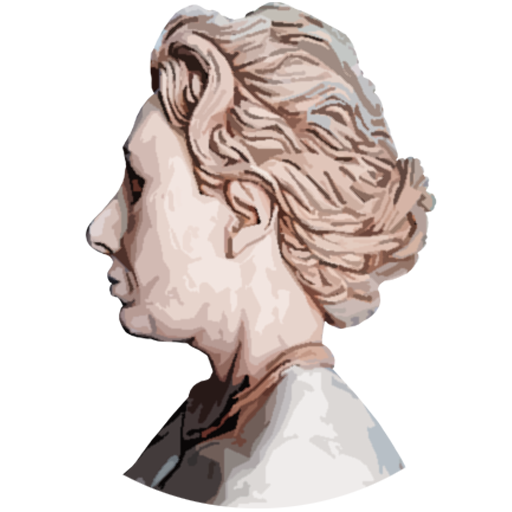
\includegraphics[width=3cm]{imagenes/logo} 
\vspace{0.5cm}

{\Huge\bfseries \myTitle \\}
\noindent\rule[-1ex]{\textwidth}{3pt}\\[3.5ex]
{\large\bfseries \mySubtitle \\[4cm]}
\end{minipage}

\vspace{2.5cm}

\noindent\hspace*{\centeroffset}
\begin{minipage}{\textwidth}
\centering
\textbf{Autor}\\ {\myName}\\[2.5ex]
\textbf{Director}\\ {\myProf}\\[2cm]
\end{minipage}

\vspace{\stretch{2}}

\end{titlepage}




\cleardoublepage
\thispagestyle{empty}

\begin{center}
{\large\bfseries \myTitle: \mySubtitle}\\
\end{center}

\begin{center}
\myName \\
\end{center}

\vspace{0.7cm}
\noindent{\textbf{Palabras clave}: informática gráfica, volúmenes, filtros, segmentación, tomografía computarizada, escultura policromada de madera, conservación y restauración, restaurador de arte}\\

\vspace{0.7cm}
\noindent{\textbf{Resumen}}\\

Tras resolver el problema del renderizado de conjuntos de datos volumétricos y crear un software sencillo para estas tareas, se pretende continuar el desarrollo de éste enfocándose en otros tres objetivos claros. Dos de ellos son completar las otras dos fases de modelado de volúmenes previas al renderizado: el filtrado y la segmentación. Y el otro es proveer al software de herramientas para poder realizar tareas de documentación por parte de los usuarios finales de éste. En cuanto al filtrado, se van a proporcionar filtros básicos de reducción de ruido para no renderizar los datos en crudo que nos devuelve el escáner. El problema de segmentación que se tratará de resolver será el de dividir la figura en los distintos trozos de madera que la conforman. Por último se creará un entorno de documentación integrado en el software para poder realizar cualquier apunte dentro de la aplicación. Se integrarán widgets para realizar medidas de distancias y ángulos y para hacer anotaciones de texto en distintos cortes generados. Todas estas tareas se dividirán en distintas tareas y se seguirá un desarrollo ágil usando las herramientas que proporciona GitHub para la gestión de un proyecto. Una vez terminado el desarrollo se realizarán una serie de pruebas y se documentarán los resultados obtenidos.

\thispagestyle{empty}

\cleardoublepage

\begin{center}
	{\large\bfseries \myTitle: \myEnglishSubtitle}\\
\end{center}

\begin{center}
	\myName \\
\end{center}

\vspace{0.7cm}
\noindent{\textbf{Keywords}: Computer Graphics, Volume, Filtering, Segmentation, Computed Tomography, Polychromed Wood Sculpture, Conservation-Restoration of Cultural Heritage, Art Curator}\\

\vspace{0.7cm}
\noindent{\textbf{Abstract}}\\

After solving the problem of volume rendering and build an application to do these tasks we will continue the development focusing on three well-differentiated objectives. Filtering, segmentation and to provide the software of tools in order to make documentation tasks by the final user. To solve the filtering objective we will provide basic reduction noise filters to apply the volumetric dataset before rendering it. Regarding the segmentation, we will try to solve the problem of dividing the original figure into the different pieces of wood it is composed by. Finally we will build an integrated documentation environment in the software. We will also integrate widgets to make measurements of distances and angles and to make text annotations in different generated slices. All these tasks will be divided into sub-tasks and we will follow an agile development by using the tools provided by GitHub to manage the project. Once we finish the development, we will make some tests and we will documentate the obtained results.

\chapter*{}
\thispagestyle{empty}

\noindent\rule[-1ex]{\textwidth}{2pt}\\[4.5ex]

Yo, \textbf{\myName}, alumno de la titulación \myDegree de la \textbf{\myFaculty}, con DNI 75926571Y, autorizo la ubicación de la siguiente copia de mi Trabajo Fin de Máster en la biblioteca del centro para que pueda ser consultada por las personas que lo deseen.

\vspace{6cm}

\noindent Fdo: \myName

\vspace{2cm}

\begin{flushright}
\myLocation a \myTime.
\end{flushright}


\chapter*{}
\thispagestyle{empty}

\noindent\rule[-1ex]{\textwidth}{2pt}\\[4.5ex]

D. \textbf{\myProf}, Profesor del Área de Lenguajes y Sistemas Informáticos del \myDepartment de la \myUni.

\vspace{0.5cm}

\textbf{Informa:}

\vspace{0.5cm}

Que el presente trabajo, titulado \textit{\textbf{\myTitle, \mySubtitle}}, ha sido realizado bajo su supervisión por \textbf{\myName}, y autorizamos la defensa de dicho trabajo ante el tribunal que corresponda.

\vspace{0.5cm}

Y para que conste, expiden y firman el presente informe en \myLocation a \myTime.

\vspace{1cm}

\textbf{El director:}

\vspace{5cm}

\noindent \textbf{\myProf}

\chapter*{Agradecimientos}
\thispagestyle{empty}

\vspace{1cm}

En primer lugar, agradecer a todos aquellos que han hecho esto posible: 
\\

A mi tutor, Javier Melero, que confió en mi para este proyecto cuando hace ya casi tres años fui a su despacho en busca de un trabajo de fin de grado que ha podido ser continuado como trabajo fin de máster. 
\\

Al Portal Virtual de Patrimonio de las Universidades Andaluzas por la cesión de los modelos de las esculturas de Inmaculada Concepción y San Juan Evangelista que han sido utilizadas para probar el software. 
\\

Y a Concha y Amparo de Artemisia Gestión de Patrimonio por ofrecerme parte de su tiempo y proporcionar su conocimiento del tema.
\\

Por otra parte, también querría que tuviesen un apartado en esta sección ese grupo fantástico de compañeros que he tenido durante el máster. 
\\

Y cómo no, a todos los que me han animado a seguir cuando apenas quedaban fuerzas.
\frontmatter
\tableofcontents
\listoffigures
\listoftables

\mainmatter
\setlength{\parskip}{5pt}

\chapter{Introducción}

Este trabajo de fin de máster es una continuación del trabajo de fin de grado que realicé en el que se desarrolló un \textit{software} (3DCurator) para visualizar un conjunto de datos volumétricos, en formato DICOM, de esculturas de madera policromada.

Con este \textit{software}, los expertos en la materia como restauradores o historiadores del arte podían inspeccionar el interior de las esculturas sin dañarlas para un posterior proceso de estudio, restauración y/o conservación.

En este trabajo de fin de máster se llevarán a cabo distintas tareas de desarrollo que se integrarán a 3DCurator así como un estudio teórico más completo del proceso de obtención de datos volumétricos en los objetos que abarcan el campo de estudio en cuestión.

Las tareas de desarrollo que se integrarán con el \textit{software} desarrollado se dividen en tres bloques:

\begin{itemize}
	\item \textbf{Pre-procesamiento de datos}: Se estudiarán los distintos filtros disponibles para ver cuáles ofrecen mejores resultados en la tarea de reducción de ruido.
	\item \textbf{Subdivisión de piezas de madera}: Las esculturas suelen estar formadas por distintas piezas de madera. Se estudiará la forma de segmentarla probando, en primer lugar, los algoritmos ya existentes utilizados principalmente en medicina. Si ninguno ofrece los resultados que esperamos, se pasará a desarrollar uno propio.
	\item \textbf{Herramientas de documentación}: Se incluirán herramientas para ayudar a los usuarios en la tarea de documentación permitiendo, por ejemplo, incluir distintas anotaciones en puntos de interés.
\end{itemize}

Además de las librerías que ya se utilizaron: VTK \cite{vtk} (visualización), Qt \cite{qt} (GUI) y Boost \cite{boost} (XML); se utilizarán las librerías ITK \cite{itk} y OpenCV \cite{opencv} para el análisis de imágenes y la visión por computador respectivamente. Haciendo uso de CMake \cite{cmake} para pre-compilarlas todas juntas.

Antes de empezar a profundizar en aspectos técnicos se realizará una introducción al proceso de obtención de datos volumétricos usando una Tomografía Computarizada así como de los objetos que se quieren analizar con esta técnica de obtención de datos: las esculturas de madera policromada.

\section{Tomografía Computarizada}

\subsection{Historia}

La tomografía computarizada (TC) es una técnica de obtención de imágenes muy utilizado en el campo de la medicina para, por ejemplo, localizar y ver el tamaño de tumores.

Sus orígenes se remontan a los años 60 cuando en 1967 Goodfrey Newblod Hounsfield propuso la elaboración del que llamó escáner EMI, base para desarrollar el Tomógrafo Axial Computarizado (TAC). El objetivo era ``\textit{crear una imagen tridimensional de un objeto tomando múltiples mediciones del mismo con la misma fuente de rayos X desde diferentes ángulos y utilizar un ordenador que permita reconstruir a partir de cientos de `planos' superpuestos y entrecruzados}'' \cite{gonzales11}.

Cuatro años más tarde, en 1971, se realizó con éxito el primer escáner cerebral usando este tomógrafo. En 1972 se instaló permanentemente en el hospital donde realizaron las pruebas y al año siguiente ya era solicitado por hospitales alrededor de todo el mundo.

\subsection{Generaciones}

El sistema de tomografía computarizada ha pasado por cuatro generaciones \cite{sarrio16}:

\subsubsection{Primera generación}

La adquisición de datos en la primera generación se basaba en la geometría del haz de rayos X paralelo y traslación-rotación en un tubo de rayos X y un solo detector (Figura \ref{fig:introduccion/primera-generacion}). El haz de rayos X se colimaba en dimensiones de 2 x 13mm. Estos 13mm correspondían al grosor del corte. Se tomaba una medida por cada 160 rotaciones durante 180 traslaciones dando un total de 28.800 medidas. El proceso era lento, tardaba unos 5 minutos, y el movimiento del paciente afectaba muy negativamente a la calidad de la imagen, por lo que su uso se veía reducido al escaneo de zonas que podían mantenerse inmóviles como la cabeza.

\begin{figure}[H]
	\centering
	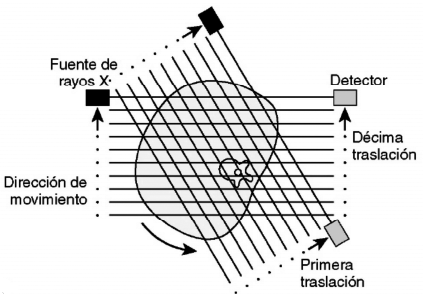
\includegraphics[width=10cm]{imagenes/introduccion/primera-generacion}
	\caption{Primera generación de aparatos de tomografía computarizada \cite{garcia14}}
	\label{fig:introduccion/primera-generacion}
\end{figure}

\subsubsection{Segunda generación}

En esta segunda generación se aumentó el número de detectores (de 5 a 30) por lo que se vio disminuido el tiempo de la exploración a unos 18 segundos (Figura \ref{fig:introduccion/segunda-generacion}).

\begin{figure}[H]
	\centering
	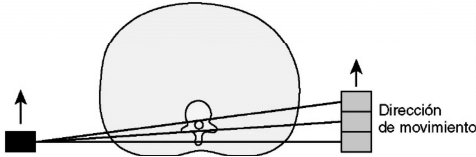
\includegraphics[width=10cm]{imagenes/introduccion/segunda-generacion}
	\caption{Segunda generación de aparatos de tomografía computarizada \cite{garcia14}}
	\label{fig:introduccion/segunda-generacion}
\end{figure}

\subsubsection{Tercera generación}

La tercera generación supuso un gran cambio y se ha convertido en la configuración estándar utilizada en la mayoría de los sistemas de escáner. Se utiliza una geometría de haz en abanico de gran angular (50º a 55º), un arco de detectores y un tubo de rayos X. Estos elementos giran 360º alrededor del paciente (Figura \ref{fig:introduccion/tercera-generacion}). El número de detectores se encuentra entre 600 y 900. Con este sistema el tiempo de barrido oscila entre 3 y 10 segundos.

\begin{figure}[H]
	\centering
	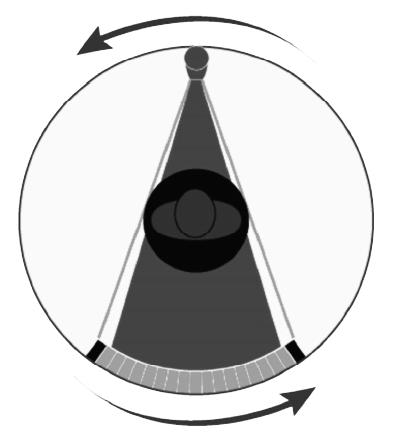
\includegraphics[width=6cm]{imagenes/introduccion/tercera-generacion}
	\caption{Tercera generación de aparatos de tomografía computarizada \cite{garcia14}}
	\label{fig:introduccion/tercera-generacion}
\end{figure}

\subsubsection{Cuarta generación}

La cuarta generación es muy parecida a la tercera solo que añade una configuración de giro estacionario (Figura \ref{fig:introduccion/cuarta-generacion}).

\begin{figure}[H]
	\centering
	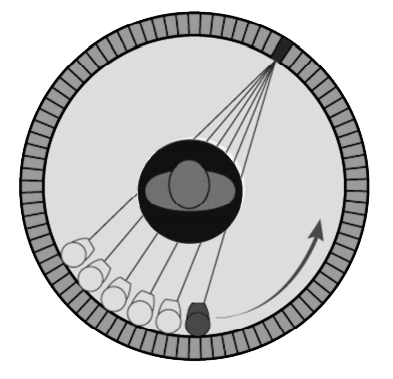
\includegraphics[width=6cm]{imagenes/introduccion/cuarta-generacion}
	\caption{Cuarta generación de aparatos de tomografía computarizada \cite{garcia14}}
	\label{fig:introduccion/cuarta-generacion}
\end{figure}

\subsubsection{Nuevas tecnologías}

\begin{itemize}
	\item \textbf{TC helicoidal (TCH)}: Hasta finales de los años 80, los aparatos de TC adquirían los datos en cortes según un método conocido como exploración axial (de ahí el nombre de TAC). Con los sistemas de tipo helicoidal los datos se obtienen de forma continua mientras se avanza la mesa a través del \textit{gantry} haciendo que el tubo de rayos X describa una trayectoria helicoidal (Figura \ref{fig:introduccion/tch}).
	
	\begin{figure}[H]
		\centering
		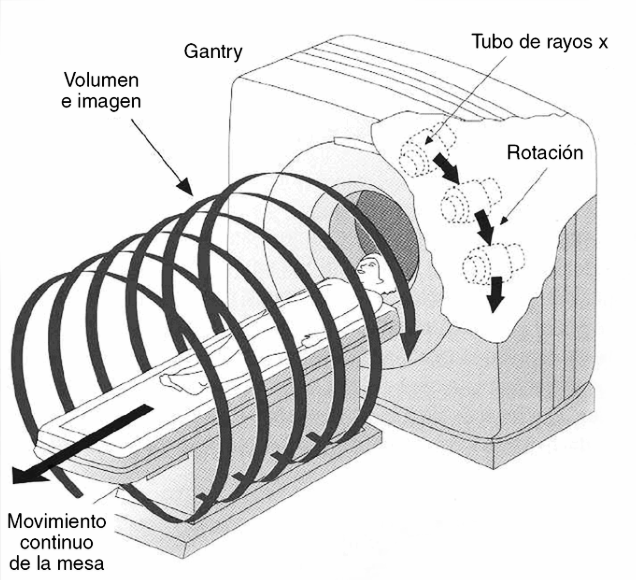
\includegraphics[width=9cm]{imagenes/introduccion/tch}
		\caption{Cuarta generación de aparatos de tomografía computarizada \cite{garcia14}}
		\label{fig:introduccion/tch}
	\end{figure}
	
	\item \textbf{TC helicoidal multicorte (TCM)}: En el lugar donde había una fila de detectores, se colocan múltiples filas. Los primeros tenían 4 filas contiguas, pero posteriormente se ha pasado a alrededor de 16 y 64 filas (Figura \ref{fig:introduccion/tcm}). Por cada rotación se estudia un mayor volumen aumentando así la velocidad de rotación y por tanto los tiempos de exposición obteniendo imágenes de mayor calidad.
	
	\begin{figure}[H]
		\centering
		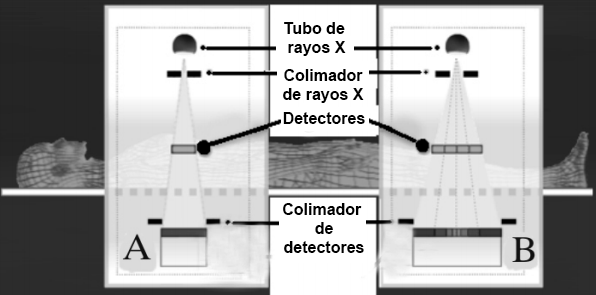
\includegraphics[width=10cm]{imagenes/introduccion/tcm}
		\caption{Diferencias entre TC helicoidal multicorte (B) y monocorte (A) \cite{sarrio16}}
		\label{fig:introduccion/tcm}
	\end{figure}

	\item \textbf{TC de doble fuente (TCED)}: Es uno de los equipos más novedosos pues permiten realizar estudios con diferentes espectros de rayos X. Utilizan dos tubos de rayos X colocados de forma perpendicular en el \textit{gantry} (Figura \ref{fig:introduccion/tced}). Se obtiene por tanto una resolución temporal equivalente a un cuarto del tiempo de rotación del \textit{gantry}.
	
	\begin{figure}[H]
		\centering
		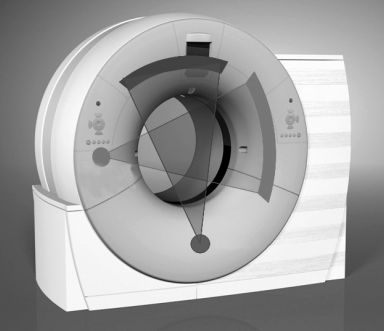
\includegraphics[width=9cm]{imagenes/introduccion/tced}
		\caption{Equipo TC con doble fuente \cite{sarrio16}}
		\label{fig:introduccion/tced}
	\end{figure}

\end{itemize}



\section{Esculturas de madera policromadas}

\subsection{Historia}

El tallado es el método de elaboración de esculturas más antiguo conocido. Se ha tallado en distintos materiales (madera, piedra, marfil...). Pero la madera, por condiciones como su ligereza o la facilidad de ensamblado entre distintas piezas, ha sido uno de los materiales más utilizados.

Se conoce que desde el Antiguo Egipto ya se realizaban esculturas de madera pero es a partir del siglo XI cuando comienza su proliferación. Y desde este momento comienzan a producirse mejoras en las técnicas y herramientas utilizadas durante el proceso del tallado \cite{sarrio16}.

\subsection{Maderas más utilizadas}

Dependiendo del tipo de escultura se utilizan maderas blandas o duras. Si la escultura es más pequeña y contiene más detalles se utilizará un tipo de madera más dura.

No obstante, en la elección también tiene mucha influencia la situación geográfica al utilizarse maderas autóctonas \cite{sarrio16}:

\begin{itemize}
	\item \textbf{Italia}: Álamo y chopo.
	\item \textbf{Francia}: Nogal y castaño.
	\item \textbf{Países Bajos}: Roble y encina.
	\item \textbf{España}: Pino de Flandes, cedro de la Habana, castaño, tejo, álamo, nogal, ciprés, boj, pino silvestre y algunos frutales como el peral.
\end{itemize}

Además de la madera, una escultura de madera policromada, puede contener varios materiales como el estuco o el metal de los clavos utilizados.

\subsection{Defectos de la madera}

Entre los defectos de la madera se pueden encontrar \cite{sarrio16}:

\subsubsection{Grietas o fendas}
Según la UNE-EN 844-9 se denomina grieta o fenda a ``toda separación de las fibras (raja o hendidura) en dirección longitudinal". Según su origen, pueden ser de distintos tipos: 

\begin{itemize}
	\item \textbf{Acebolladuras o \textit{colainas}}: Hay una discontinuidad entre los anillos de crecimiento.
	\item \textbf{Superficiales o de desecación}: Producidas por el calor, provocan un deterioro en las zonas externas del tronco del árbol dejando la madera desprotegida. Provocan grietas en sentido longitudinal.
	\item \textbf{De heladura}: Producidas por una helada dañan la superficie e interior del tronco. Provocan grietas radiales.
	\item \textbf{De viento}: Originadas por la acción de un fuerte viento. Provocan grietas longitudinales y transversales.
\end{itemize}

Además de estos procesos naturales, se pueden producir grietas durante procesos como el secado que provocan una separación de las fibras.

\subsubsection{Fibras reviradas y entrelazadas}

Las fibras se encuentran normalmente orientadas en paralelo al eje principal del tronco, pero en ocasiones pueden presentar nudos que alteran la dirección de éstas.

\subsubsection{Nudos}

La UNE 56.521 define nudo como ``anomalía local de la estructura de la madera producida por la parte inferior de una rama que va quedando englobada en el tronco a medida que se producen los crecimientos de este". Existen distintos tipos:

\begin{itemize}
	\item \textbf{Adherente, vivo, fijo o sano}: Definido por la UNE 56.521 como ``aquel cuyos tejidos son solidarios con los de la madera que los rodea debido a ser formado por una rama viva".
	\item \textbf{Suelto, saltadizo, muerto o seco}: Definido por la UNE 56.521 como ``aquel en que los tejidos de la rama que lo producen no son solidarios con los de la madera que los rodea y suelen separarse".
\end{itemize}

\subsubsection{Núcleos de resina}

Son cavidades entre los anillos de crecimiento producidos frecuentemente por nudos.

\subsubsection{Factores de deterioro de tipo biótico}

Además de las alteraciones que ya presenta la madera, existen otros factores que también influyen como la humedad y la temperatura o el ataque de insectos xilófagos y hongos.

Los insectos xilófagos se nutren de madera seca y favorecen a su desarrollo una humedad relativa y temperaturas no muy bajas. Estos producen daños rompiendo las fibras de la madera.

Los hongos son microorganismos que pueden desarrollarse en la superficie o en el interior de la madera, haciendo que pierda humedad, reduciendo su tamaño y deformándose. Existen tres tipos distintos de degradación tras un ataque de hongos: pudrición blanca, parda o seca y blanda.

\subsection{Proceso de tallado}

El proceso de tallado se podría definir como una técnica sustractiva en la que a partir de una pieza se obtiene una forma concreta.

Un método puede ser utilizar un único bloque de madera. En ocasiones ahuecado por el reverso para contrarrestar fuerza y movimiento de la madera, y, en cierto modo, aligerando el peso.

A partir del siglo XVI empieza a utilizarse con más frecuencia otro método en el que a partir de un bloque principal se ensamblan diferentes piezas generando un bloque más grande, denominado embón, con la forma y el tamaño de la imagen a esculpir. A partir de éste se comienza el tallado.

A partir del Barroco se mejora esta técnica realizando ensamblados en hueco para evitar el posterior ahuecado \cite{sarrio16}.

\section{Estado del arte}

Como ya se ha comentado anteriormente, este trabajo es la continuación del trabajo fin de grado que realicé. Durante este trabajo fin de grado resolví el problema de la visualización de datos volumétricos de esculturas de madera policromada \cite{bolivar16}. Pero no realizaba ningún pre-procesamiento, tan solo se visualizaban permitiendo explorar la escultura en su interior. Toda la información que obtenía el experto que usase el programa debía ser anotada a mano a parte pues tampoco se proporcionaba funcionalidad para almacenar esta información para poder ser rescatada posteriormente.

Este trabajo se divide en tres bloques: pre-procesamiento, documentación y segmentación. 

Los dos primeros están incluidos en la mayoría de los programas disponibles en la web de visualización de datos volumétricos. Tales como AMILab \cite{krissian12}, RadiAnt \cite{radiant}, Slicer \cite{fedorov12} o el usado por María Francisca en su estudio \cite{sarrio16} OsiriX \cite{rosset04} en el que me he inspirado para realizar mi implementación. Todas estas herramientas son muy completas, pero los resultados obtenidos al visualizar los datos volumétricos de esculturas de madera policromadas dejaban mucho que desear y el gran número de funciones específicas para la medicina los hacen complejos de más, y es que por esta razón surgió la idea de crear un software específico de visualización de datos volumétricos de esculturas.

El tercer bloque, el de la segmentación, es totalmente novedoso pues no hay ningún tipo de segmentación específica para separar distintos trozos de madera. Sin embargo, antes de programar un algoritmo específico habría que probar con los que ya hay disponibles que además son muy usados en el campo de la medicina.

Existen varias aproximaciones para llevar a cabo la segmentación en datos volumétricos. Pueden clasificarse en:

\begin{itemize}
	\item Segmentación manual
	\item Segmentación semi-automática
	\item Segmentación basada en umbrales (\textit{thresholding})
	\item Segmentación basada en crecimiento de regiones (\textit{region-growing})
	\item Segmentación basada en bordes (\textit{edge})
\end{itemize}

La segmentación manual la podríamos descartar automáticamente. Pese a que es un método que siempre se puede aplicar, tener a una persona recortando manualmente las distintas piezas corte por corte puede ser muy costoso en cuanto a tiempo.

Los métodos de segmentación basada en umbrales \cite{otsu79} se basan en definir un umbral en los valores escalares de cada vóxel para diferenciar las distintas partes del volumen. Estos no nos son útiles pues las distintas piezas de madera suelen ser del mismo material y coincidir en estos valores de densidad.

Los métodos de segmentación basada en crecimiento de regiones que utilizan umbrales \cite{haralick85} tampoco nos van a servir pues las distintas piezas de madera se encuentran juntas. Otros métodos de segmentación basada en regiones como la transformación divisoria (\textit{watershed}) \cite{beucher79} tampoco nos van a servir pues se definirían muchas cuencas debido a los anillos que presentan los cortes de la madera y si se empiezan a inundar para obtener regiones más grandes obtendremos un resultado similar al que obtenemos con el de crecimiento de regiones con umbrales.

Los métodos de segmentación basados en bordes como el \textit{livewire} \cite{mortensen95} podrían resultar efectivos pues el borde que separa dos piezas de madera es visualmente diferenciable. No obstante, este método necesita de una supervisión humana y, aunque sea más preciso y rápido que una segmentación manual, se debería seguir realizando corte a corte.

Como vemos, ninguno de los métodos que no requieren de supervisión humana son efectivos a la hora de resolver nuestro problema. Es por ello que, definitivamente, hay que desarrollar uno propio.
\chapter{Especificación de requisitos}

Este capítulo es una Especificación de Requisitos Software para el software que se va a realizar siguiendo las directrices dadas por el estándar IEEE830 \cite{iee830}.

\section{Introducción}

\subsection{Propósito}

Este capítulo de especificación de requisitos tiene como objetivo definir las especificaciones funcionales y no funcionales para el desarrollo de un software que permitirá pre-procesar datos DICOM obtenidos al someter a una escultura de madera policromada a una TC para que posteriormente los usuarios puedan realizar labores de documentación al explorar la figura así como realizar una segmentación de los distintos trozos de madera que la componen. 

\subsection{Ámbito del sistema}

En la actualidad, los datos DICOM obtenidos tras una TC se utilizan, principalmente, en el campo donde surgieron, la medicina. Con este software llamado 3DCurator, se tratará de trasladar esta técnica al campo de la restauración de bienes culturales y poder pre-procesar, visualizar, interactuar y documentar los datos DICOM obtenidos con esculturas de madera policromada.

\subsection{Definiciones, acrónimos y abreviaturas}

\begin{itemize}
	\item \textbf{ERS} (Especificación de Requisitos Software).
	\item \textbf{GUI} (Interfaz Gráfica de usuario).
	\item \textbf{\textit{Widget}}: Elemento de la GUI.
	\item \textbf{DICOM} (\textit{Digital Imaging and Communication in Medicine}): Formato de datos volumétricos donde se obtienen las imágenes.
	\item \textbf{CT o TC} (Tomografía Computarizada): Técnica de extracción de datos volumétricos que utiliza radiación X para obtener cortes de objetos.
	\item \textbf{MRI o IRM} (Imagen por Resonancia Magnética): Técnica de extracción de datos volumétricos que utiliza el fenómeno de resonancia magnética nuclear.
	\item \textbf{PET} (Tomografía por Emisión de Positrones): Técnica de extracción de datos volumétricos capaz de medir la actividad metabólica del cuerpo humano.
	\item \textbf{CPU} (\textit{Graphic Processor Unit}): Microprocesador.
	\item \textbf{GPU} (\textit{Graphic Processor Unit}): Tarjeta gráfica.
	\item \textbf{UML} (Lenguaje unificado de modelado): Lenguaje de modelado de sistemas software.
	\item \textbf{Historia de usuario}: Representación de un requisito utilizando el lenguaje común del usuario.
	\item \textbf{\textit{Product Backlog}}: Listado de historias de usuario del proyecto.
	\item \textbf{C++}: Lenguaje de programación que se usará.
	\item \textbf{XML} (\textit{Extension Markup Language}): Meta lenguaje que se usará para exportar ficheros que después podrán ser importados.
	\item \textbf{CMake} (\textit{Cross platform Make}): Herramienta para generar código compilable en distintas plataformas.
	\item \textbf{Qt}: Librería que se utilizará para realizar la GUI.
	\item \textbf{VTK} (\textit{The Visualization ToolKit}): Librería gráfica que se utilizará para la visualización de volúmenes.
	\item \textbf{ITK} (\textit{Insight Segmentation and Registration Toolkit}): Librería de procesamiento de imágenes que se utilizará.
	\item \textbf{OpenCV}: Librería de visión por computador que se utilizará.
	\item \textbf{Boost}: Conjunto de algoritmos para C++ de los que se usarán la gestión de ficheros XML.
	\item \textbf{Volumen}: Conjunto de datos en los que para cada posición XYZ se tiene un valor determinado.
	\item \textbf{\textit{Voxel}} (\textit{Volumentric Pixel}): Celda en la matriz 3D del conjunto de datos del volumen.
	\item \textbf{Vecinadario}: Celdas alrededor de un voxel.
	\item \textbf{Adyacencia de voxels}: Voxels vecinos que satisfacen un criterio de similitud.
	\item \textbf{Conectividad de voxels}: Voxels entre los cuales hay un camino de voxels adyacentes.
	\item \textbf{Malla}: Estructura de datos con la información de una superficie tridimensional.
	\item \textbf{STL} (\textit{Standard Triangle Language}): Formato que define mallas 3D.
	\item \textbf{Corte}: Vista de la figura a través de un plano. Por ejemplo, al cortar con una sierra un tronco por la mitad, se puede ver cómo es por dentro en esa posición por donde se ha cortado.
	\item \textbf{TF} (Función de transferencia): Función utilizada para visualizar los datos deseados de un volumen.
	\item \textbf{\textit{Preset}}: Función de transferencia previamente configurada.
	\item \textbf{\textit{Direct Volume Rendering}}: Visualización directa de volúmenes en la que cada valor del volumen se mapea con un determinado color y opacidad dado por una función de transferencia.
	\item \textbf{\textit{Ray Casting}}: Técnica de \textit{Direct Volume Rendering} utilizada para la visualización de volúmenes.
	\item \textbf{\textit{Marching Cubes}}: Técnica para generar malla de polígonos a partir de un volumen y un valor de isosuperficie.
	\item \textbf{HU} (\textit{Hounsfield Units}): Unidad de medida escalar del valor de densidad en un \textit{voxel} del volumen.
	\item \textbf{ROD} (\textit{Región de documentación}): Corte en el que se documentará.
	\item \textbf{Regla}: \textit{Widget} utilizado para realizar mediciones de distancias.
	\item \textbf{Transportador de ángulos}: \textit{Widget} utilizado para realizar mediciones de ángulos.
	\item \textbf{Nota}: \textit{Widget} utilizado para realizar anotaciones sobre la figura.
	\item \textbf{Segmentación}: Método por el cual se distinguen distintas partes del volumen.
	\item \textbf{\textit{Thresholding}}: Segmentación basada en umbrales.
	\item \textbf{\textit{Region-growing}}: Segmentación basada en crecimiento de regiones.
	\item \textbf{Semilla}: Coordenada donde se comienza el \textit{region-growing}.
	\item \textbf{\textit{Watershed}}: Técnica de segmentación basada en crecimiento de regiones por inundación.
	\item \textbf{\textit{Canny Edge Detection}}: Algoritmo para resaltar los bordes de una imagen.
	\item \textbf{Transformada de Hough}: Técnica utilizada para detectar líneas rectas.
	\item \textbf{Filtro gaussiano}: Filtro que utiliza la distribución gaussiana del vecindario.
	\item \textbf{Filtro media}: Filtro que utiliza la media del vecindario.
	\item \textbf{Filtro mediana}: Filtro que utiliza la mediana del vecindario.
	\item \textbf{Embón}: Ensamblado de distintos trozos de madera que hacen de base para la escultura.
	\item \textbf{Estuco}: Pasta de grano fino utilizada para realizar correcciones en la escultura.
	\item \textbf{Policromía}: Capa de pintura de las esculturas.
	\item \textbf{Blanco de plomo}: Pigmento de color blanco creado a partir del plomo.
	\item \textbf{Pan de oro}: Lámina muy fina de oro.
\end{itemize}

\subsection{Visión general del documento}

Este capítulo consta de tres secciones:
\begin{itemize}
	\item En la primera sección se realiza una introducción a éste y se proporciona una visión general de la ERS.
	\item En la segunda sección se realiza una descripción general a alto nivel del software, describiendo los factores que afectan al producto y a sus requisitos y con el objetivo de conocer las principales funcionalidades de éste.
	\item En la tercera sección se definen detalladamente los requisitos que deberá satisfacer el software.
\end{itemize}

\section{Descripción general}

\subsection{Perspectiva del producto}

El software 3DCurator tiene como objetivo interactuar con datos DICOM, pero no es el encargado de generarlos. Para generarlos se deberá utilizar algún escáner de TC.

Una vez obtenidos, se podrán pre-procesar aplicando una serie de filtros, segmentar en los distintos trozos de madera que forman la escultura y documentar añadiendo notas y mediciones de distancias y ángulos.

\subsection{Funciones del producto}

Las principales funcionalidades de este sistema serán:

\begin{itemize}
	\item Pre-procesar la imagen aplicando filtros de reducción de ruido:
	\begin{itemize}
		\item Media.
		\item Mediana.
		\item Gaussiano.
	\end{itemize}
	\item Documentar la escultura:
	\begin{itemize}
		\item Agregar anotación.
		\item Agregar regla.
		\item Agregar transportador de ángulos.
	\end{itemize}
	\item Segmentar la escultura por los distintos trozos de madera.
	\item Exportar el volumen segmentado.
\end{itemize}

\subsection{Características de los usuarios}

Solo existe un tipo de usuario, que es la persona que desee interactuar con los datos DICOM de una escultura. Esta persona no tiene por qué tener habilidad con un equipo informático, por lo que \myTitle deberá tener una GUI intuitiva y fácil de utilizar.

\chapter{Planificación}

En este capítulo se comentará la planificación inicial de tiempo en la que se llevará a cabo este TFM, la estimación en horas de cada módulo de tareas, la metodología de trabajo, los resultados y los presupuestos.

\section{Planificación temporal inicial}

La fecha de inicio trabajando en el proyecto que me fijé es el 1 de diciembre de 2016 y se espera llegar a la convocatoria de julio de 2017 por lo que se cuentan con siete meses. No obstante, y como es lógico, no voy a trabajar exclusivamente en este proyecto durante estos meses pues tengo que cursar el resto de asignaturas del máster, además debería tener un mes de margen para pulir la memoria desarrollando algunas secciones y organizando lo que haya ido apuntando durante el resto de meses. Por lo que serían 6 meses de desarrollo.

Para organizarme he decidido dedicar un número de horas semanales al desarrollo de este proyecto. Inicialmente me he fijado 15 horas a la semana dando un total de 360 horas de desarrollo puro excluyendo la redacción de la memoria.

Ordenando los módulos por prioridades y dependencias se tendría la siguiente planificación:

\begin{longtable} {l c c c}
	\hline
	\textbf{Tarea}			&	\textbf{Duración}	&	\textbf{Comienzo}	&	\textbf{Fin}	\\
	\hline \hline
	\endhead
	\hline 
	Exportación/importación	&	2 semanas			&	01/12/2016			&	14/12/2016		\\
	\hline
	Filtrado				&	6 semanas			&	15/12/2016			&	25/01/2017		\\
	\hline
	Segmentación			&	10 semanas			&	26/01/2017			&	05/04/2017		\\
	\hline
	Documentación			&	8 semanas			&	06/04/2017			&	31/05/2017		\\
	\hline
	Mejoras					&	1 semana			&	01/06/2017			&	07/06/2017		\\
	\hline
	Memoria					&	4 semanas			&	08/06/2017			&	05/07/2017		\\
	\hline
	\\
	\caption{Planificación inicial}
	\label{tab:planificacion/planificacion-inicial}
\end{longtable}

\subsection{Diagrama de Gantt}

Aunque el diagrama de Gantt tiene más sentido cuando se pueden paralelizar tareas y al haber un único desarrollador esto no es posible, realicé este diagrama porque de un vistazo se ve más clara la planificación que con la tabla anterior.

\begin{figure}[H]
	\centering
	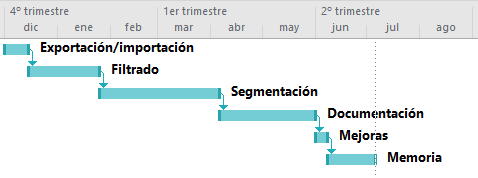
\includegraphics[width=12cm]{imagenes/planificacion/gantt}
	\caption{Diagrama de Gantt con la planficación inicial del proyecto generado con \textit{Microsoft Office Project 2016}}
	\label{fig:planificacion/gantt}
\end{figure}


\section{Metodología de trabajo}

\subsection{\textit{GitHub}}

Aprovechando que se está usando \textit{git} como sistema de control de versiones en un repositorio de \textit{GitHub}, voy a aprovechar todos los recursos que nos ofrece esta plataforma para organizarme. 

\subsection{\textit{Issues}}

En lugar de tener por un lado un tablero \textit{kanban} (por ejemplo \textit{Trello}), yo voy a utilizar los \textit{issues} (Figura \ref{fig:planificacion/issues}) de mi repositorio en \textit{GitHub} para organizar las tareas, así como ir añadiendo tareas nuevas que vaya necesitando y tener un registro de qué he hecho y cuándo, que problemas han surgido, etc.

\begin{figure}[H]
	\centering
	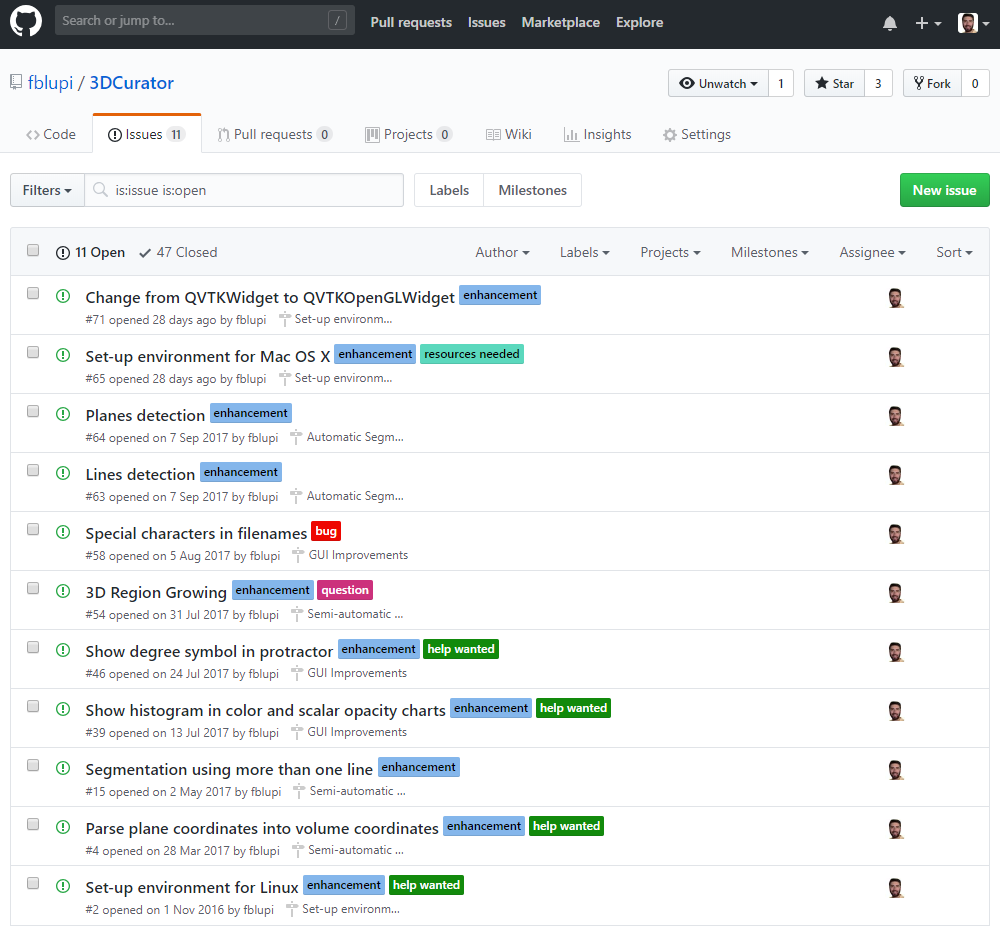
\includegraphics[width=12cm]{imagenes/planificacion/issues}
	\caption{Vista con la lista de \textit{issues} abiertos con sus correspondientes etiquetas y el \textit{milestone} al que pertenecen}
	\label{fig:planificacion/issues}
\end{figure}

Una de las ventajas de utilizar los \textit{issues} de \textit{GitHub} antes que otra plataforma como \textit{Trello} es la posibilidad de referenciarlos en los \textit{commit} agregando \texttt{\#ref} en el mensaje. Y dentro del propio \textit{issue} se vería una lista de todos los \textit{commit} donde se ha trabajado en éste. Además, si antes de escribir la referencia del \textit{issue} se añade \texttt{closes}, el \textit{issue} se cerrará automáticamente sin necesidad de hacerlo de forma manual.

\subsection{\textit{Milestones}}

Voy a clasificar los \textit{issues} por \textit{milestones} (Figura \ref{fig:planificacion/milestones}), uno por cada módulo y al mismo tiempo voy a agregarles \textit{tags} para etiquetarlos según sean \textit{bugs}, mejoras, bloqueantes por necesidad de recursos o por ayuda necesitada, etc.

\begin{figure}[H]
	\centering
	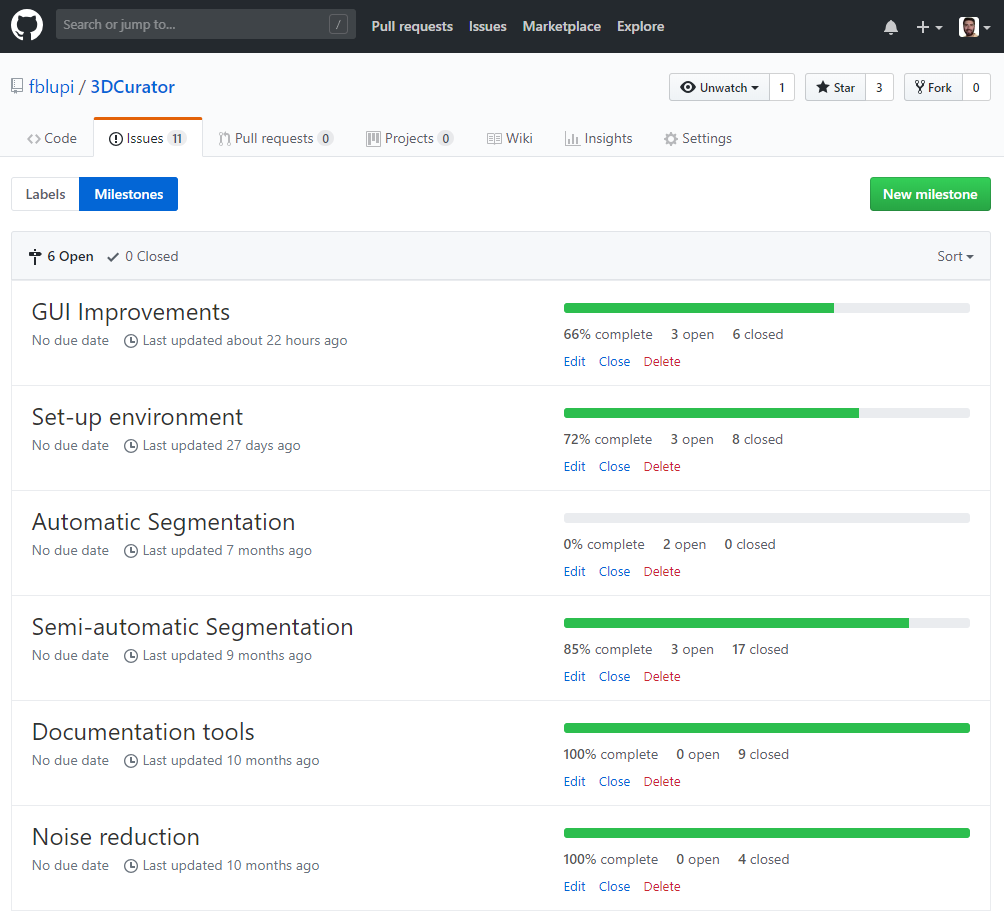
\includegraphics[width=12cm]{imagenes/planificacion/milestones}
	\caption{Resumen de los \textit{milestones} con su porcentaje de elaboración}
	\label{fig:planificacion/milestones}
\end{figure}

\subsection{\textit{Branches}}

La organización que voy a llevar en cuanto a las ramas (\textit{branches}), es la siguiente, basada en \textit{Gitflow} \cite{gitflow}:

\begin{itemize}
	\item \textbf{\textit{master}}: Esta rama tendrá la última \textit{release} del programa. Debe ser completamente estable, pues es de donde se generan los instaladores finales de la aplicación.
	\item \textbf{\textit{develop}}: Esta es la rama principal con los últimos cambios desarrollados (Figura \ref{fig:planificacion/commits}). Cuando se tiene una batería de cambios suficiente como para generar una nueva versión del \textit{software} se realizará un \textit{pull request} a \textit{master} por lo que esta rama debe ser también estable.
	\item \textbf{\textit{features}}: Estas son ramas de trabajo que no tienen por qué ser estables. Por ejemplo, si se va a agregar un filtro \textit{gaussiano} se podría crear una rama con el nombre \textit{feature/gaussian-filter} y trabajar en esta rama hasta que se validase esta nueva funcionalidad. Entonces se haría un \textit{rebase} con \textit{develop} por si ha habido algún cambio durante el transcurso de este desarrollo para resolver conflictos y finalmente un \textit{pull request} a \textit{develop} para mezclar los cambios.
\end{itemize}

Además cuento con otras ramas auxiliares que no intervienen en el flujo de desarrollo pero donde almaceno información útil.

\begin{itemize}
	\item \textbf{\textit{design}}: En esta rama se encuentran los diagramas de paquetes y clases actualizados con la versión del software en la rama \textit{develop}.
	\item \textbf{\textit{assets}}: En esta rama se almacenan recursos como logos e imágenes utilizados en la aplicación.
	\item \textbf{\textit{user-manual}}: En esta rama se encuentra el manual de usuario de la aplicación.
	\item \textbf{\textit{gh-pages}}: En esta rama se encuentra la \textit{landing page} de la aplicación. Pues \textit{GitHub} ofrece gratuitamente alojamiento para una página web estática por repositorio.
\end{itemize}

\begin{figure}[H]
	\centering
	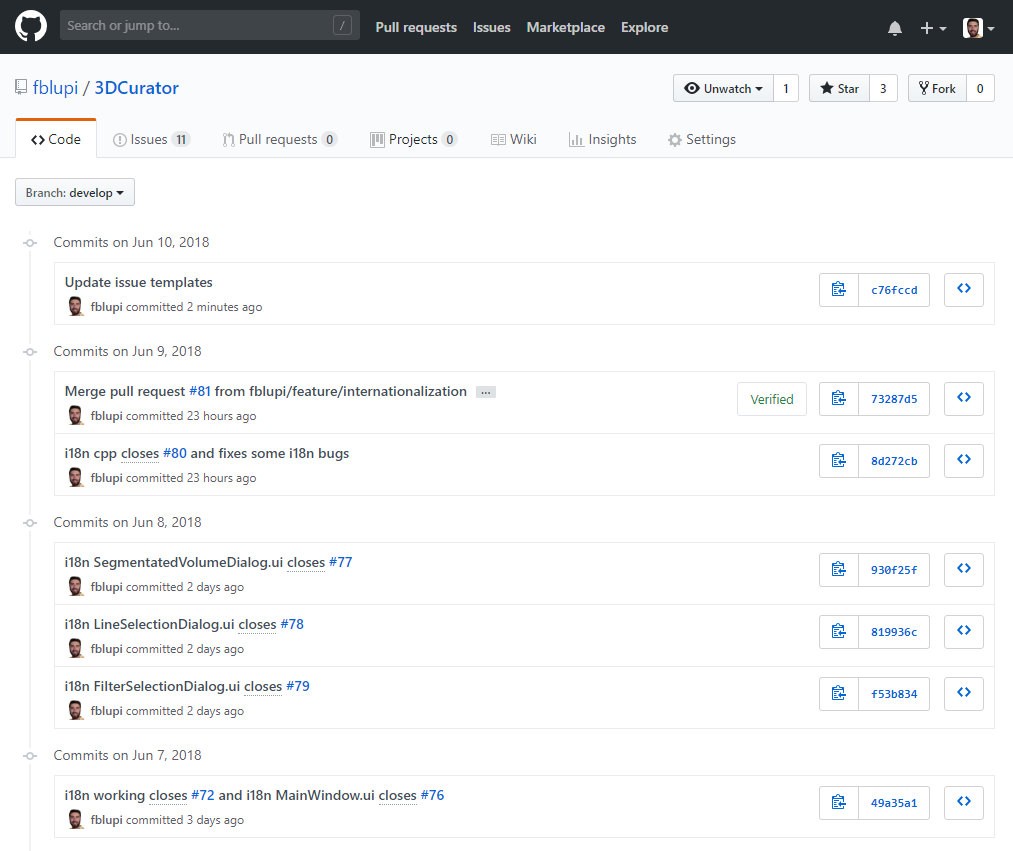
\includegraphics[width=12cm]{imagenes/planificacion/commits}
	\caption{Ejemplo de \textit{commits} en la rama \textit{develop}}
	\label{fig:planificacion/commits}
\end{figure}

\section{Resultados}

Los resultados no tienen nada que ver con la planificación inicial que se hizo. La carga del trabajo del resto de asignaturas del máster han hecho que le dedicase muchas menos horas a la semana que las que tenía pensado y durante algunos periodos lo he tenido que tener apartado.

Cuando llegó junio y vi que no llegaba a la convocatoria, recalculé tiempos para llegar a septiembre. Pero otra vez se vieron trastocados pues en agosto empecé a trabajar a jornada completa y las horas que le pude echar se volvieron a ver reducidas. No obstante llegué a tenerlo todo a excepción de la documentación. Que ya, una vez matriculado de nuevo en la asignatura la tomé con calma.

Además, me permití el lujo de añadir a última hora internacionalización al proyecto para poder tener la aplicación también en inglés además de la versión ya existente en español.

\begin{figure}[H]
	\centering
	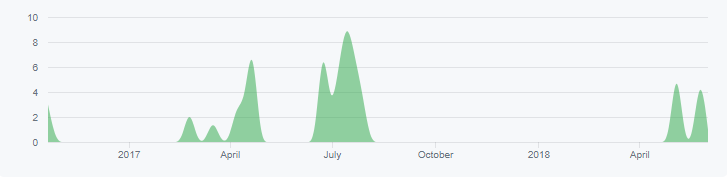
\includegraphics[width=12cm]{imagenes/planificacion/resultados}
	\caption{Gráfico de los \textit{commits} realizados en la rama \textit{develop}. El gráfico es orientativo porque hay \textit{commits} con poca funcionalidad y otros con mucha, pero ayuda a ver las etapas donde más se trabajó}
	\label{fig:planificacion/resultados}
\end{figure}

En total he registrado 312 horas de desarrollo frente a las 360 planificadas. Esto quiere decir que la planificación de tareas no ha fallado como tal. La que ha fallado ha sido la planificación de disponibilidad de recursos humanos.

\section{Presupuestos}

Este proyecto tiene costes tanto en recursos físicos como en recursos humanos. Se desglosan a continuación:

\begin{itemize}
	\item \textbf{Equipo de trabajo}: Ordenador portátil MSI CX61 2PC cuyo coste inicial es de 800 \euro{} pero tiene una vida de 4 años y al ser usado durante año y medio tendría un coste de: $ 800 \times 1.5 / 4 = 300 $
	\item \textbf{Tomografías}: El costo que tuvieron tanto la cesión como la tomografía de ambas figuras fueron de 90 \euro{} por unidad dando un total de $ 90 \times 2 = 180 $
	\item \textbf{Ingeniero informático}: El coste por hora de un ingeniero informático con mi cualificación ronda ahora mismo en el mercado laboral los 10 \euro{}/hora por lo que tendría un coste de: $ 10 \times 360 = 3600 $
	\item \textbf{Asesor}: Mi tutor hará de asesor y aproximadamente dedicará unas 36 horas entre reuniones y revisiones. Estimo unos 20 \euro{}/hora dando un total de $ 20 \times 36 = 720$
\end{itemize}

El coste total del proyecto sería de 4800 \euro{}. Se puede ver como gran parte de este presupuesto (el 92,08\%) va dedicado a recursos humanos.
\chapter{Análisis}

En este capítulo se describirán las distintas historias de usuario que han sido implementadas en el software.

\section{Historias de usuario}

\subsection{\textit{Product backlog}}

A continuación se muestra el listado de historias de usuario (\textit{Product Backlog}) completo separadas por módulo, y para cada historia de usuario sus dependencias, estimación (en puntos de historia) y prioridad.

\begin{longtable} {r l c c c}
	\hline
	\#	&	\textbf{Descripción}					&	\textbf{Dep.}	&	\textbf{Est.}	&	\textbf{Prio.}	\\
	\hline \hline
	\endhead
	\multicolumn{5}{l}{\textbf{Auxiliar}} \\
	\hline 
	1.1.	&	Exportar volumen					&	-				&	12				&	1	\\
	\hline
	1.2.	&	Importar volumen					&	1.1.			&	8				&	5	\\
	\hline
	\multicolumn{5}{l}{\textbf{Pre-procesamiento}} \\
	\hline 
	2.1.	&	Filtro \textit{gaussiano}			&	-				&	24				&	1	\\
	\hline
	2.2.	&	Filtro media						&	-				&	10				&	3	\\
	\hline
	2.3.	&	Filtro mediana						&	-				&	8				&	3	\\
	\hline
	\multicolumn{5}{l}{\textbf{Segmentación}} \\
	\hline 
	3.1.	&	Segmentar pieza de madera			&	1.1.			&	64				&	1	\\
	\hline
	\multicolumn{5}{l}{\textbf{Documentación}} \\
	\hline 
	4.1.	&	Crear ROD							&	-				&	4				&	1	\\
	\hline
	4.2.	&	Eliminar ROD						&	4.1.			&	4				&	3	\\
	\hline
	4.3.	&	Exportar ROD						&	4.1.			&	2				&	2	\\
	\hline
	4.4.	&	Importar ROD						&	4.3.			&	3				&	2	\\
	\hline
	4.5.	&	Cambiar ROD							&	4.1.			&	3				&	1	\\
	\hline
	4.6.	&	Crear regla							&	-				&	3				&	2	\\
	\hline
	4.7.	&	Eliminar regla						&	4.6				&	3				&	4	\\
	\hline
	4.8.	&	Editar regla						&	4.6				&	1				&	5	\\
	\hline
	4.9.	&	Ocultar regla						&	4.6				&	2				&	6	\\
	\hline
	4.10.	&	Mostrar regla						&	4.9				&	1				&	6	\\
	\hline
	4.11.	&	Crear transportador de ángulos		&	-				&	3				&	3	\\
	\hline
	4.12.	&	Eliminar transportador de ángulos	&	4.11.			&	3				&	5	\\
	\hline
	4.13.	&	Editar transportador de ángulos		&	4.11.			&	1				&	6	\\
	\hline
	4.14.	&	Ocultar transportador de ángulos	&	4.11.			&	2				&	7	\\
	\hline
	4.15.	&	Mostrar transportador de ángulos	&	4.14.			&	1				&	7	\\
	\hline
	4.16.	&	Crear nota							&	-				&	4				&	2	\\
	\hline
	4.17.	&	Eliminar nota						&	4.16.			&	2				&	4	\\
	\hline
	4.18.	&	Editar nota							&	4.16.			&	3				&	5	\\
	\hline
	4.19.	&	Ocultar nota						&	4.16.			&	2				&	6	\\
	\hline
	4.20.	&	Mostrar nota						&	4.19.			&	1				&	6	\\
	\hline
	\multicolumn{5}{l}{\textbf{Mejoras en código}} \\
	\hline
	5.1.	&	Internacionalización				&	-				&	6				&	8	\\
	\hline
	\\
	\caption{Historias de usuario}
	\label{tab:analisis/hus}
\end{longtable}

Se han estimado un total de 180 PH (Puntos de historia) y se habían planificado unas 360 horas de trabajo. Por lo que cada PH corresponde aproximadamente a 2 horas.

Al haber registrado 312 horas finalmente, he determinado que mi velocidad ha sido aproximadamente 1,73 horas/PH, un poco más rápido que lo planificado.

\subsection{Tarjetas de las historias de usuario}

A continuación se incluye una descripción completa de las historias de usuario incluyendo una descripción de ésta y sus correspondientes criterios de aceptación.

\subsubsection{Auxiliar}

\begin{table}[H]
	\begin{center}
		\begin{tabular} {l|c|l}
			\hline
			1.1. & \multicolumn{2}{c}{Exportar volumen} \\ \noalign{\hrule height 1pt}
			\multicolumn{3}{l}{Descripción} \\ \hline
			\multicolumn{3}{p{12cm}}{Se debe proveer a la aplicación de la funcionalidad necesaria para exportar el volumen que se ha cargado y editado para poder utilizarlo de nuevo posteriormente sin tener que volver a editarlo. Para ello se tratará de utilizar el formato propio de VTK para almacenar volúmenes, VTI, que hace uso de XML. Se le mostrará al usuario un diálogo donde elegirá la carpeta y el nombre del archivo.} \\ \noalign{\hrule height 1pt}
			\multicolumn{2}{l|}{Estimación} & 12 \\ \hline
			\multicolumn{2}{l|}{Prioridad} & 1 \\ \hline
			\multicolumn{2}{l|}{Dependencias} & - \\ \noalign{\hrule height 1pt}
			\multicolumn{3}{l}{Pruebas de aceptación} \\ \hline
			\multicolumn{3}{p{12cm}}{ - El usuario realiza la acción de exportar sin ningún volumen cargado y le aparece un mensaje para que lo cargue antes.} \\
			\multicolumn{3}{p{12cm}}{ - El usuario no elige nombre y se guardará el archivo con un nombre por defecto ne la carpeta elegida.} \\ 
			\multicolumn{3}{p{12cm}}{ - El usuario elige el nombre y se guardará el archivo con el nombre elegido en la carpeta elegida.} \\ 
			\hline
		\end{tabular}
	\end{center}
	\caption{Historia de usuario - Exportar volumen}
	\label{tab:analisis/hu-exportar-volumen}
\end{table}

\begin{table}[H]
	\begin{center}
		\begin{tabular} {l|c|l}
			\hline
			1.2. & \multicolumn{2}{c}{Importar volumen} \\ \noalign{\hrule height 1pt}
			\multicolumn{3}{l}{Descripción} \\ \hline
			\multicolumn{3}{p{12cm}}{El \textit{software} debe poder leer ficheros en formato VTI como los previamente exportados. Para ello el usuario deberá poder elegir un archivo en un diálogo donde se filtrarán los ficheros para que se muestren solo los que tienen la extensión VTI.} \\ \noalign{\hrule height 1pt}
			\multicolumn{2}{l|}{Estimación} & 8 \\ \hline
			\multicolumn{2}{l|}{Prioridad} & 5 \\ \hline
			\multicolumn{2}{l|}{Dependencias} & 1.1. \\ \noalign{\hrule height 1pt}
			\multicolumn{3}{l}{Pruebas de aceptación} \\ \hline
			\multicolumn{3}{p{12cm}}{ - Si el usuario lee un archivo que no es VTI no lo podrá visualizar.} \\
			\multicolumn{3}{p{12cm}}{ - Si el usuario elige un archivo VTI correcto se importará y podrá empezar a utilizarlo.} \\ \hline
		\end{tabular}
	\end{center}
	\caption{Historia de usuario - Importar volumen}
	\label{tab:analisis/hu-importar-volumen}
\end{table}

\subsubsection{Pre-procesamiento}

\begin{table}[H]
	\begin{center}
		\begin{tabular} {l|c|l}
			\hline
			2.1. & \multicolumn{2}{c}{Filtro \textit{gaussiano}} \\ \noalign{\hrule height 1pt}
			\multicolumn{3}{l}{Descripción} \\ \hline
			\multicolumn{3}{p{12cm}}{Se debe poder aplicar un filtro \textit{gaussiano} al volumen para reducir el ruido. Para ello el usuario elegirá el número de repeticiones que se realizarán (de 1 a 5). Se utilizará la librería ITK para aplicar este filtro.} \\ \noalign{\hrule height 1pt}
			\multicolumn{2}{l|}{Estimación} & 24 \\ \hline
			\multicolumn{2}{l|}{Prioridad} & 1 \\ \hline
			\multicolumn{2}{l|}{Dependencias} & - \\ \noalign{\hrule height 1pt}
			\multicolumn{3}{l}{Pruebas de aceptación} \\ \hline
			\multicolumn{3}{p{12cm}}{ - El usuario filtra sin haber ningún volumen cargado y le aparece un mensaje de que cargue antes un modelo.} \\
			\multicolumn{3}{p{12cm}}{ - El usuario selecciona el filtrado y los parámetros deseados y se realiza el filtrado en el volumen, el resultado será un volumen más suavizado.} \\ \hline
		\end{tabular}
	\end{center}
	\caption{Historia de usuario - Filtro \textit{gaussiano}}
	\label{tab:analisis/hu-filtro-gaussiano}
\end{table}

\begin{table}[H]
	\begin{center}
		\begin{tabular} {l|c|l}
			\hline
			2.2. & \multicolumn{2}{c}{Filtro media} \\ \noalign{\hrule height 1pt}
			\multicolumn{3}{l}{Descripción} \\ \hline
			\multicolumn{3}{p{12cm}}{Se debe poder aplicar un filtro media al volumen para reducir ruido. Para ello el usuario elegirá el tamaño del vecindario (3x3, 5x5 o 7x7). Se utilizará la librería ITK para aplicar este filtro.} \\ \noalign{\hrule height 1pt}
			\multicolumn{2}{l|}{Estimación} & 10 \\ \hline
			\multicolumn{2}{l|}{Prioridad} & 3 \\ \hline
			\multicolumn{2}{l|}{Dependencias} & - \\ \noalign{\hrule height 1pt}
			\multicolumn{3}{l}{Pruebas de aceptación} \\ \hline
			\multicolumn{3}{p{12cm}}{ - El usuario filtra sin haber ningún volumen cargado y le aparece un mensaje de que cargue antes un modelo.} \\
			\multicolumn{3}{p{12cm}}{ - El usuario selecciona el filtrado y los parámetros deseados y se realiza el filtrado en el volumen, el resultado será un volumen más suavizado.} \\ \hline
		\end{tabular}
	\end{center}
	\caption{Historia de usuario - Filtro media}
	\label{tab:analisis/hu-filtro-media}
\end{table}

\begin{table}[H]
	\begin{center}
		\begin{tabular} {l|c|l}
			\hline
			2.3. & \multicolumn{2}{c}{Filtro mediana} \\ \noalign{\hrule height 1pt}
			\multicolumn{3}{l}{Descripción} \\ \hline
			\multicolumn{3}{p{12cm}}{Se debe poder aplicar un filtro mediana al volumen para reducir ruido. Para ello el usuario elegirá el tamaño del vecindario (3x3, 5x5 o 7x7). Se utilizará la librería ITK para aplicar este filtro.} \\ \noalign{\hrule height 1pt}
			\multicolumn{2}{l|}{Estimación} & 8 \\ \hline
			\multicolumn{2}{l|}{Prioridad} & 3 \\ \hline
			\multicolumn{2}{l|}{Dependencias} & - \\ \noalign{\hrule height 1pt}
			\multicolumn{3}{l}{Pruebas de aceptación} \\ \hline
			\multicolumn{3}{p{12cm}}{ - El usuario filtra sin haber ningún volumen cargado y le aparece un mensaje de que cargue antes un modelo.} \\
			\multicolumn{3}{p{12cm}}{ - El usuario selecciona el filtrado y los parámetros deseados y se realiza el filtrado en el volumen. Esto reducirá el ruido de tipo \textit{salt-and-pepper}.} \\ \hline
		\end{tabular}
	\end{center}
	\caption{Historia de usuario - Filtro mediana}
	\label{tab:analisis/hu-filtro-mediana}
\end{table}

\subsubsection{Segmentación}

\begin{table}[H]
	\begin{center}
		\begin{tabular} {l|c|l}
			\hline
			3.1. & \multicolumn{2}{c}{Segmentar pieza de madera} \\ \noalign{\hrule height 1pt}
			\multicolumn{3}{l}{Descripción} \\ \hline
			\multicolumn{3}{p{12cm}}{El usuario debe poder separar las distintas piezas de madera de las que está compuesta la figura. Para ello se desarrollará un método semi-automático guiado por el usuario para partir en dos un volumen, de forma iterativa se podría realizar la descomposición total de la figura. El usuario elegirá en el visor de corte el trozo deseado a segmentar y el sistema le preguntará por cuál de las posibles líneas detectadas divide las piezas de madera, el usuario le responderá y el sistema terminará el proceso. Para realizar esto se deberán combinar filtros, técnicas de visión por computador y de segmentación de volúmenes.} \\ \noalign{\hrule height 1pt}
			\multicolumn{2}{l|}{Estimación} & 64 \\ \hline
			\multicolumn{2}{l|}{Prioridad} & 1 \\ \hline
			\multicolumn{2}{l|}{Dependencias} & 1.1. \\ \noalign{\hrule height 1pt}
			\multicolumn{3}{l}{Pruebas de aceptación} \\ \hline
			\multicolumn{3}{p{12cm}}{ - El usuario elige una pieza de madera y la línea que la separa y se devolverá un volumen con esta pieza.} \\ \hline
		\end{tabular}
	\end{center}
	\caption{Historia de usuario - Segmentar pieza de madera}
	\label{tab:analisis/hu-segmentar-pieza-de-madera}
\end{table}

\subsubsection{Documentación}

\begin{table}[H]
	\begin{center}
		\begin{tabular} {l|c|l}
			\hline
			4.1. & \multicolumn{2}{c}{Crear ROD} \\ \noalign{\hrule height 1pt}
			\multicolumn{3}{l}{Descripción} \\ \hline
			\multicolumn{3}{p{12cm}}{Se debe poder crear un área de trabajo de documentación, es decir, imágenes donde incluir anotaciones. Para ello se ha creado el concepto ROD (Region of Documentation), que no es más que una posición del plano de corte donde se podrán incluir medidas y anotaciones. El usuario colocará el plano en la posición deseada y creará una ROD a la que podrá dar nombre, si no, cogerá un nombre por defecto.} \\ \noalign{\hrule height 1pt}
			\multicolumn{2}{l|}{Estimación} & 4 \\ \hline
			\multicolumn{2}{l|}{Prioridad} & 1 \\ \hline
			\multicolumn{2}{l|}{Dependencias} & - \\ \noalign{\hrule height 1pt}
			\multicolumn{3}{l}{Pruebas de aceptación} \\ \hline
			\multicolumn{3}{p{12cm}}{ - El usuario crea una ROD sin nombre y se guarda la posición del plano con un nombre por defecto.} \\
			\multicolumn{3}{p{12cm}}{ - El usuario crea una ROD con nombre y se guarda la posición del plano con el nombre indicado.} \\ \hline
		\end{tabular}
	\end{center}
	\caption{Historia de usuario - Crear ROD}
	\label{tab:analisis/hu-crear-rod}
\end{table}

\begin{table}[H]
	\begin{center}
		\begin{tabular} {l|c|l}
			\hline
			4.2. & \multicolumn{2}{c}{Eliminar ROD} \\ \noalign{\hrule height 1pt}
			\multicolumn{3}{l}{Descripción} \\ \hline
			\multicolumn{3}{p{12cm}}{El usuario debe poder eliminar una ROD creada con anterioridad. Para ello la selecciona y pulsa en la opción de eliminar.} \\ \noalign{\hrule height 1pt}
			\multicolumn{2}{l|}{Estimación} & 4 \\ \hline
			\multicolumn{2}{l|}{Prioridad} & 3 \\ \hline
			\multicolumn{2}{l|}{Dependencias} & 4.1. \\ \noalign{\hrule height 1pt}
			\multicolumn{3}{l}{Pruebas de aceptación} \\ \hline
			\multicolumn{3}{p{12cm}}{ - No hay ninguna ROD seleccionada, el usuario pulsa en eliminar y le aparece un mensaje de que debe seleccionar antes una.} \\
			\multicolumn{3}{p{12cm}}{ - El usuario selecciona una ROD, la elimina y desaparece del listado de ROD.} \\ \hline
		\end{tabular}
	\end{center}
	\caption{Historia de usuario - Eliminar ROD}
	\label{tab:analisis/hu-eliminar-rod}
\end{table}

\begin{table}[H]
	\begin{center}
		\begin{tabular} {l|c|l}
			\hline
			4.3. & \multicolumn{2}{c}{Exportar ROD} \\ \noalign{\hrule height 1pt}
			\multicolumn{3}{l}{Descripción} \\ \hline
			\multicolumn{3}{p{12cm}}{Se tiene que proveer al sistema de la funcionalidad necesaria para poder exportar una ROD con todos sus componentes de forma que pueda volver a importarlo. Para ello se exportará en formato XML.} \\ \noalign{\hrule height 1pt}
			\multicolumn{2}{l|}{Estimación} & 2 \\ \hline
			\multicolumn{2}{l|}{Prioridad} & 2 \\ \hline
			\multicolumn{2}{l|}{Dependencias} & 4.1. \\ \noalign{\hrule height 1pt}
			\multicolumn{3}{l}{Pruebas de aceptación} \\ \hline
			\multicolumn{3}{p{12cm}}{ - No hay ninguna ROD seleccionada, el usuario pulsa en exportar y le aparece un mensaje de que debe seleccionar antes una.} \\
			\multicolumn{3}{p{12cm}}{ - El usuario exporta una ROD seleccionada, elige el nombre, que por defecto es su nombre y se guarda correctamente en formato XML.} \\ \hline
		\end{tabular}
	\end{center}
	\caption{Historia de usuario - Exportar ROD}
	\label{tab:analisis/hu-exportar-rod}
\end{table}

\begin{table}[H]
	\begin{center}
		\begin{tabular} {l|c|l}
			\hline
			4.4. & \multicolumn{2}{c}{Importar ROD} \\ \noalign{\hrule height 1pt}
			\multicolumn{3}{l}{Descripción} \\ \hline
			\multicolumn{3}{p{12cm}}{Se debe poder leer un archivo XML con un formato específico con información de una ROD y sus componentes. Para ello se le mostrará al usuario un cuadro de diálogo donde explorará entre sus archivos, realizando un filtrado para mostrar solo los ficheros XML} \\ \noalign{\hrule height 1pt}
			\multicolumn{2}{l|}{Estimación} & 3 \\ \hline
			\multicolumn{2}{l|}{Prioridad} & 2 \\ \hline
			\multicolumn{2}{l|}{Dependencias} & 4.3. \\ \noalign{\hrule height 1pt}
			\multicolumn{3}{l}{Pruebas de aceptación} \\ \hline
			\multicolumn{3}{p{12cm}}{ - El usuario carga un archivo con el formato válido y se importa la ROD con todos sus componentes.} \\ \hline
		\end{tabular}
	\end{center}
	\caption{Historia de usuario - Importar ROD}
	\label{tab:analisis/hu-importar-rod}
\end{table}

\begin{table}[H]
	\begin{center}
		\begin{tabular} {l|c|l}
			\hline
			4.5. & \multicolumn{2}{c}{Cambiar ROD} \\ \noalign{\hrule height 1pt}
			\multicolumn{3}{l}{Descripción} \\ \hline
			\multicolumn{3}{p{12cm}}{El usuario debe poder cambiar la ROD activa seleccionándola dentro de la lista de ROD. Esto cambiará automáticamente la posición del plano para usar la de esta ROD.} \\ \noalign{\hrule height 1pt}
			\multicolumn{2}{l|}{Estimación} & 3 \\ \hline
			\multicolumn{2}{l|}{Prioridad} & 1 \\ \hline
			\multicolumn{2}{l|}{Dependencias} & 4.1. \\ \noalign{\hrule height 1pt}
			\multicolumn{3}{l}{Pruebas de aceptación} \\ \hline
			\multicolumn{3}{p{12cm}}{ - El usuario selecciona la misma ROD que está activa y no cambia.} \\
			\multicolumn{3}{p{12cm}}{ - El usuario selecciona una ROD que no está activa y cambia la posición del plano y se muestran los elementos de esa ROD.} \\ \hline
		\end{tabular}
	\end{center}
	\caption{Historia de usuario - Cambiar ROD}
\label{tab:analisis/hu-cambiar-rod}
\end{table}

\begin{table}[H]
	\begin{center}
		\begin{tabular} {l|c|l}
			\hline
			4.6. & \multicolumn{2}{c}{Crear regla} \\ \noalign{\hrule height 1pt}
			\multicolumn{3}{l}{Descripción} \\ \hline
			\multicolumn{3}{p{12cm}}{.} \\ \noalign{\hrule height 1pt}
			\multicolumn{2}{l|}{Estimación} & 3 \\ \hline
			\multicolumn{2}{l|}{Prioridad} & 2 \\ \hline
			\multicolumn{2}{l|}{Dependencias} & - \\ \noalign{\hrule height 1pt}
			\multicolumn{3}{l}{Pruebas de aceptación} \\ \hline
			\multicolumn{3}{p{12cm}}{ - .} \\ \hline
		\end{tabular}
	\end{center}
	\caption{Historia de usuario - Crear regla}
	\label{tab:analisis/hu-crear-regla}
\end{table}

\begin{table}[H]
	\begin{center}
		\begin{tabular} {l|c|l}
			\hline
			4.7. & \multicolumn{2}{c}{Eliminar regla} \\ \noalign{\hrule height 1pt}
			\multicolumn{3}{l}{Descripción} \\ \hline
			\multicolumn{3}{p{12cm}}{.} \\ \noalign{\hrule height 1pt}
			\multicolumn{2}{l|}{Estimación} & 3 \\ \hline
			\multicolumn{2}{l|}{Prioridad} & 4 \\ \hline
			\multicolumn{2}{l|}{Dependencias} & 4.6. \\ \noalign{\hrule height 1pt}
			\multicolumn{3}{l}{Pruebas de aceptación} \\ \hline
			\multicolumn{3}{p{12cm}}{ - .} \\ \hline
		\end{tabular}
	\end{center}
	\caption{Historia de usuario - Eliminar regla}
	\label{tab:analisis/hu-eliminar-regla}
\end{table}

\begin{table}[H]
	\begin{center}
		\begin{tabular} {l|c|l}
			\hline
			4.8. & \multicolumn{2}{c}{Editar regla} \\ \noalign{\hrule height 1pt}
			\multicolumn{3}{l}{Descripción} \\ \hline
			\multicolumn{3}{p{12cm}}{.} \\ \noalign{\hrule height 1pt}
			\multicolumn{2}{l|}{Estimación} & 1 \\ \hline
			\multicolumn{2}{l|}{Prioridad} & 5 \\ \hline
			\multicolumn{2}{l|}{Dependencias} & 4.6. \\ \noalign{\hrule height 1pt}
			\multicolumn{3}{l}{Pruebas de aceptación} \\ \hline
			\multicolumn{3}{p{12cm}}{ - .} \\ \hline
		\end{tabular}
	\end{center}
	\caption{Historia de usuario - Editar regla}
	\label{tab:analisis/hu-editar-regla}
\end{table}

\begin{table}[H]
	\begin{center}
		\begin{tabular} {l|c|l}
			\hline
			4.9. & \multicolumn{2}{c}{Ocultar regla} \\ \noalign{\hrule height 1pt}
			\multicolumn{3}{l}{Descripción} \\ \hline
			\multicolumn{3}{p{12cm}}{.} \\ \noalign{\hrule height 1pt}
			\multicolumn{2}{l|}{Estimación} & 2 \\ \hline
			\multicolumn{2}{l|}{Prioridad} & 6 \\ \hline
			\multicolumn{2}{l|}{Dependencias} & 4.6. \\ \noalign{\hrule height 1pt}
			\multicolumn{3}{l}{Pruebas de aceptación} \\ \hline
			\multicolumn{3}{p{12cm}}{ - .} \\ \hline
		\end{tabular}
	\end{center}
	\caption{Historia de usuario - Ocultar regla}
	\label{tab:analisis/hu-ocultar-regla}
\end{table}

\begin{table}[H]
	\begin{center}
		\begin{tabular} {l|c|l}
			\hline
			4.10. & \multicolumn{2}{c}{Mostrar regla} \\ \noalign{\hrule height 1pt}
			\multicolumn{3}{l}{Descripción} \\ \hline
			\multicolumn{3}{p{12cm}}{.} \\ \noalign{\hrule height 1pt}
			\multicolumn{2}{l|}{Estimación} & 1 \\ \hline
			\multicolumn{2}{l|}{Prioridad} & 6 \\ \hline
			\multicolumn{2}{l|}{Dependencias} & 4.9. \\ \noalign{\hrule height 1pt}
			\multicolumn{3}{l}{Pruebas de aceptación} \\ \hline
			\multicolumn{3}{p{12cm}}{ - .} \\ \hline
		\end{tabular}
	\end{center}
	\caption{Historia de usuario - Mostrar regla}
	\label{tab:analisis/hu-mostrar-regla}
\end{table}

\begin{table}[H]
	\begin{center}
		\begin{tabular} {l|c|l}
			\hline
			4.11. & \multicolumn{2}{c}{Crear transportador de ángulos} \\ \noalign{\hrule height 1pt}
			\multicolumn{3}{l}{Descripción} \\ \hline
			\multicolumn{3}{p{12cm}}{.} \\ \noalign{\hrule height 1pt}
			\multicolumn{2}{l|}{Estimación} & 3 \\ \hline
			\multicolumn{2}{l|}{Prioridad} & 3 \\ \hline
			\multicolumn{2}{l|}{Dependencias} & - \\ \noalign{\hrule height 1pt}
			\multicolumn{3}{l}{Pruebas de aceptación} \\ \hline
			\multicolumn{3}{p{12cm}}{ - .} \\ \hline
		\end{tabular}
	\end{center}
	\caption{Historia de usuario - Crear transportador de ángulos}
	\label{tab:analisis/hu-crear-transportador-angulos}
\end{table}

\begin{table}[H]
	\begin{center}
		\begin{tabular} {l|c|l}
			\hline
			4.12. & \multicolumn{2}{c}{Eliminar transportador de ángulos} \\ \noalign{\hrule height 1pt}
			\multicolumn{3}{l}{Descripción} \\ \hline
			\multicolumn{3}{p{12cm}}{.} \\ \noalign{\hrule height 1pt}
			\multicolumn{2}{l|}{Estimación} & 3 \\ \hline
			\multicolumn{2}{l|}{Prioridad} & 4 \\ \hline
			\multicolumn{2}{l|}{Dependencias} & 4.11. \\ \noalign{\hrule height 1pt}
			\multicolumn{3}{l}{Pruebas de aceptación} \\ \hline
			\multicolumn{3}{p{12cm}}{ - .} \\ \hline
		\end{tabular}
	\end{center}
	\caption{Historia de usuario - Eliminar transportador de ángulos}
	\label{tab:analisis/hu-eliminar-transportador-angulos}
\end{table}

\begin{table}[H]
	\begin{center}
		\begin{tabular} {l|c|l}
			\hline
			4.13. & \multicolumn{2}{c}{Editar transportador de ángulos} \\ \noalign{\hrule height 1pt}
			\multicolumn{3}{l}{Descripción} \\ \hline
			\multicolumn{3}{p{12cm}}{.} \\ \noalign{\hrule height 1pt}
			\multicolumn{2}{l|}{Estimación} & 1 \\ \hline
			\multicolumn{2}{l|}{Prioridad} & 5 \\ \hline
			\multicolumn{2}{l|}{Dependencias} & 4.11. \\ \noalign{\hrule height 1pt}
			\multicolumn{3}{l}{Pruebas de aceptación} \\ \hline
			\multicolumn{3}{p{12cm}}{ - .} \\ \hline
		\end{tabular}
	\end{center}
	\caption{Historia de usuario - Editar transportador de ángulos}
	\label{tab:analisis/hu-editar-transportador-angulos}
\end{table}

\begin{table}[H]
	\begin{center}
		\begin{tabular} {l|c|l}
			\hline
			4.14. & \multicolumn{2}{c}{Ocultar transportador de ángulos} \\ \noalign{\hrule height 1pt}
			\multicolumn{3}{l}{Descripción} \\ \hline
			\multicolumn{3}{p{12cm}}{.} \\ \noalign{\hrule height 1pt}
			\multicolumn{2}{l|}{Estimación} & 2 \\ \hline
			\multicolumn{2}{l|}{Prioridad} & 6 \\ \hline
			\multicolumn{2}{l|}{Dependencias} & 4.11. \\ \noalign{\hrule height 1pt}
			\multicolumn{3}{l}{Pruebas de aceptación} \\ \hline
			\multicolumn{3}{p{12cm}}{ - .} \\ \hline
		\end{tabular}
	\end{center}
	\caption{Historia de usuario - Ocultar transportador de ángulos}
	\label{tab:analisis/hu-ocultar-transportador-angulos}
\end{table}

\begin{table}[H]
	\begin{center}
		\begin{tabular} {l|c|l}
			\hline
			4.15. & \multicolumn{2}{c}{Mostrar transportador de ángulos} \\ \noalign{\hrule height 1pt}
			\multicolumn{3}{l}{Descripción} \\ \hline
			\multicolumn{3}{p{12cm}}{.} \\ \noalign{\hrule height 1pt}
			\multicolumn{2}{l|}{Estimación} & 1 \\ \hline
			\multicolumn{2}{l|}{Prioridad} & 7 \\ \hline
			\multicolumn{2}{l|}{Dependencias} & 4.14. \\ \noalign{\hrule height 1pt}
			\multicolumn{3}{l}{Pruebas de aceptación} \\ \hline
			\multicolumn{3}{p{12cm}}{ - .} \\ \hline
		\end{tabular}
	\end{center}
	\caption{Historia de usuario - Mostrar transportador de ángulos}
	\label{tab:analisis/hu-mostrar-transportador-angulos}
\end{table}

\begin{table}[H]
	\begin{center}
		\begin{tabular} {l|c|l}
			\hline
			4.16. & \multicolumn{2}{c}{Crear nota} \\ \noalign{\hrule height 1pt}
			\multicolumn{3}{l}{Descripción} \\ \hline
			\multicolumn{3}{p{12cm}}{.} \\ \noalign{\hrule height 1pt}
			\multicolumn{2}{l|}{Estimación} & 4 \\ \hline
			\multicolumn{2}{l|}{Prioridad} & 2 \\ \hline
			\multicolumn{2}{l|}{Dependencias} & - \\ \noalign{\hrule height 1pt}
			\multicolumn{3}{l}{Pruebas de aceptación} \\ \hline
			\multicolumn{3}{p{12cm}}{ - .} \\ \hline
		\end{tabular}
	\end{center}
	\caption{Historia de usuario - Crear nota}
	\label{tab:analisis/hu-crear-nota}
\end{table}

\begin{table}[H]
	\begin{center}
		\begin{tabular} {l|c|l}
			\hline
			4.17. & \multicolumn{2}{c}{Eliminar nota} \\ \noalign{\hrule height 1pt}
			\multicolumn{3}{l}{Descripción} \\ \hline
			\multicolumn{3}{p{12cm}}{.} \\ \noalign{\hrule height 1pt}
			\multicolumn{2}{l|}{Estimación} & 2 \\ \hline
			\multicolumn{2}{l|}{Prioridad} & 4 \\ \hline
			\multicolumn{2}{l|}{Dependencias} & 4.16. \\ \noalign{\hrule height 1pt}
			\multicolumn{3}{l}{Pruebas de aceptación} \\ \hline
			\multicolumn{3}{p{12cm}}{ - .} \\ \hline
		\end{tabular}
	\end{center}
	\caption{Historia de usuario - Eliminar nota}
	\label{tab:analisis/hu-eliminar-nota}
\end{table}

\begin{table}[H]
	\begin{center}
		\begin{tabular} {l|c|l}
			\hline
			4.18. & \multicolumn{2}{c}{Editar nota} \\ \noalign{\hrule height 1pt}
			\multicolumn{3}{l}{Descripción} \\ \hline
			\multicolumn{3}{p{12cm}}{.} \\ \noalign{\hrule height 1pt}
			\multicolumn{2}{l|}{Estimación} & 3 \\ \hline
			\multicolumn{2}{l|}{Prioridad} & 5 \\ \hline
			\multicolumn{2}{l|}{Dependencias} & 4.16. \\ \noalign{\hrule height 1pt}
			\multicolumn{3}{l}{Pruebas de aceptación} \\ \hline
			\multicolumn{3}{p{12cm}}{ - .} \\ \hline
		\end{tabular}
	\end{center}
	\caption{Historia de usuario - Editar nota}
	\label{tab:analisis/hu-editar-nota}
\end{table}

\begin{table}[H]
	\begin{center}
		\begin{tabular} {l|c|l}
			\hline
			4.19. & \multicolumn{2}{c}{Ocultar nota} \\ \noalign{\hrule height 1pt}
			\multicolumn{3}{l}{Descripción} \\ \hline
			\multicolumn{3}{p{12cm}}{.} \\ \noalign{\hrule height 1pt}
			\multicolumn{2}{l|}{Estimación} & 2 \\ \hline
			\multicolumn{2}{l|}{Prioridad} & 6 \\ \hline
			\multicolumn{2}{l|}{Dependencias} & 4.16. \\ \noalign{\hrule height 1pt}
			\multicolumn{3}{l}{Pruebas de aceptación} \\ \hline
			\multicolumn{3}{p{12cm}}{ - .} \\ \hline
		\end{tabular}
	\end{center}
	\caption{Historia de usuario - Ocultar nota}
	\label{tab:analisis/hu-ocultar-nota}
\end{table}

\begin{table}[H]
	\begin{center}
		\begin{tabular} {l|c|l}
			\hline
			4.20. & \multicolumn{2}{c}{Mostrar nota} \\ \noalign{\hrule height 1pt}
			\multicolumn{3}{l}{Descripción} \\ \hline
			\multicolumn{3}{p{12cm}}{.} \\ \noalign{\hrule height 1pt}
			\multicolumn{2}{l|}{Estimación} & 1 \\ \hline
			\multicolumn{2}{l|}{Prioridad} & 6 \\ \hline
			\multicolumn{2}{l|}{Dependencias} & 4.19. \\ \noalign{\hrule height 1pt}
			\multicolumn{3}{l}{Pruebas de aceptación} \\ \hline
			\multicolumn{3}{p{12cm}}{ - .} \\ \hline
		\end{tabular}
	\end{center}
	\caption{Historia de usuario - Mostrar nota}
	\label{tab:analisis/hu-mostrar-nota}
\end{table}

\subsubsection{Mejoras en código}

\begin{table}[H]
	\begin{center}
		\begin{tabular} {l|c|l}
			\hline
			5.1. & \multicolumn{2}{c}{Internacionalización} \\ \noalign{\hrule height 1pt}
			\multicolumn{3}{l}{Descripción} \\ \hline
			\multicolumn{3}{p{12cm}}{El usuario tiene que tener la posibilidad de utilizar la aplicación en dos idiomas distintos, español e inglés. Para ello se utilizará el mecanismo de internacionalización que provee Qt y se generarán dos instaladores: uno en español y otro en inglés.} \\ \noalign{\hrule height 1pt}
			\multicolumn{2}{l|}{Estimación} & 6 \\ \hline
			\multicolumn{2}{l|}{Prioridad} & 8 \\ \hline
			\multicolumn{2}{l|}{Dependencias} & - \\ \noalign{\hrule height 1pt}
			\multicolumn{3}{l}{Pruebas de aceptación} \\ \hline
			\multicolumn{3}{p{12cm}}{ - El usuario ejecutará el programa en cualquiera de los idiomas y se mostrarán los textos con el idioma correspondiente.} \\ \hline
		\end{tabular}
	\end{center}
	\caption{Historia de usuario - Internacionalización}
	\label{tab:analisis/hu-internacionalizacion}
\end{table}
\chapter{Diseño}

Lala
\chapter{Implementación}

Lala
\chapter{Ejemplos}

Lala
\chapter{Conclusiones y trabajos futuros}

En este último capítulo se comentarán las conclusiones a las que se han llegado así como las posibles mejoras en el futuro que se podrían realizar.

\section{Conclusiones}

Partíamos de un \textit{software} desarrollado previamente, durante el Trabajo de Fin de Grado, que permitía cargar una serie de imágenes DICOM y renderizar el volumen. Permitiendo cambiar la función de transferencia para centrarse en unos u otros materiales, realizar cortes arbitrarios para ver el interior de la figura, exportar la malla usando el método de \textit{marching cubes} y borrar partes innecesarias del volumen.

Con todo esto, un restaurador ya podía utilizar este programa y llegaría a realizar estudios mucho más completos que con otras técnicas.

No obstante, no podíamos quedarnos estancados ahí y había todavía bastantes cosas que hacer. Es por ello por lo que se decidió continuar el desarrollo de este \textit{software} durante este Trabajo de Fin de Máster.

Los objetivos los dividimos inicialmente en tres: filtrado, segmentación y documentación.

La idea principal que teníamos con el filtrado fue la de reducir el ruido producido por artefactos metálicos. No obstante no encontramos un \textit{pipeline} de filtros que lo consiguieran y vimos como otros estudios delegaban responsabilidades a la etapa del escaneo en la que, gracias a los avances en éstos y ajustándolos con parámetros adecuados, podía reducirse \cite{boas12}.

Sin embargo se integraron en el software tres filtros: \textit{gaussiano}, media y mediana, pues podrían resultar útiles tanto para suavizar imágenes ruidosas (\textit{gaussiano} y media) como para acabar con el ruido de tipo \textit{salt-and-pepper} (mediana).

La segmentación para obtener las distintas piezas de madera resultó todo un reto. Ninguno de los filtros ya existentes utilizados en medicina nos era útil y no había estudios previos que tratasen de resolver este problema.

Se fueron realizando pruebas combinando y modificando filtros ya existentes hasta que se dio con una técnica que resultó ser bastante eficaz. Estaba basada en el filtro básico de crecimiento basado en umbral, agregando una restricción más marcada por una línea. Esta línea era detectada usando técnicas de visión por computador como el filtro de \textit{Canny} y la transformada de \textit{Hough}. Y su extensión para ser usado en todos los cortes de un volumen resultaba casi trivial, pues lo único que había que buscar eran dos semillas: una donde se comienza el crecimiento, que casi siempre era la misma que la primera, y otra para generar la línea que delimitara el crecimiento, que se lograría detectando todas las líneas de ese corte y comparando similitud con la que era la línea delimitante en el corte anterior.

El método por tanto es semi-automático aunque solo necesita la interacción del usuario en dos pasos. Sin embargo es un método algo limitado pues solo sirve para dividir un volumen en dos. Aunque, no evita poder dividir en $n$ aunque habría que realizar el proceso $n-1$ veces.

Por último, la parte de documentación se preveía como la más sencilla de desarrollar. Y nada más lejos de la realidad, pues había \textit{widgets} ya presentes en la librería VTK y tan solo había que empaparse de la documentación e integrarlos en el \textit{software}.

El desarrollo de toda esta funcionalidad nueva ha permitido generar una nueva versión de esta aplicación libre y gratuita que se puede descargar para \textit{Windows} desde su \href{https://fblupi.github.io/3DCurator/es/}{web oficial}.

Todo el desarrollo se ha hecho en un \href{https://github.com/fblupi/3DCurator}{repositorio} \textit{git} alojado en \textit{GitHub}. Siguiendo una gestión de ramas basada en \textit{Gitflow} y con \textit{templates} para los \textit{issues} que hacen más sencilla la comunicación con los usuarios ya que pueden publicar su \textit{feedback} más fácilmente.

La aplicación ya cuenta con varios usuarios que han contactado conmigo dando las gracias por la aplicación y pidiendo soporte para realizar algunas tareas específicas. Sin duda, resulta satisfactorio ver cómo se puede ayudar a otro sector tan distinto a la informática con herramientas que lo pueden modernizar.

\bibliography{bibliografia/bibliografia}
\addcontentsline{toc}{chapter}{Bibliografía}
\bibliographystyle{plain}

\end{document}
